\documentclass[nohyperref]{article}

% Recommended, but optional, packages for figures and better typesetting:
\usepackage{microtype}
\usepackage{graphicx}
\usepackage{subfigure}
\usepackage{booktabs} % for professional tables

% hyperref makes hyperlinks in the resulting PDF.
% If your build breaks (sometimes temporarily if a hyperlink spans a page)
% please comment out the following usepackage line and replace
% \usepackage{icml2022} with \usepackage[nohyperref]{icml2022} above.
\usepackage{hyperref}


% Attempt to make hyperref and algorithmic work together better:
\newcommand{\theHalgorithm}{\arabic{algorithm}}

\usepackage[accepted]{icml2022}

% For theorems and such
\usepackage{amsmath}
\usepackage{amssymb}
\usepackage{mathtools}
\usepackage{amsthm}
\usepackage{listings}

% if you use cleveref..
\usepackage[capitalize,noabbrev]{cleveref}

%%%%%%%%%%%%%%%%%%%%%%%%%%%%%%%%
% THEOREMS
%%%%%%%%%%%%%%%%%%%%%%%%%%%%%%%%
\theoremstyle{plain}
\newtheorem{theorem}{Theorem}[section]
\newtheorem{proposition}[theorem]{Proposition}
\newtheorem{lemma}[theorem]{Lemma}
\newtheorem{corollary}[theorem]{Corollary}
\theoremstyle{definition}
\newtheorem{definition}[theorem]{Definition}
\newtheorem{assumption}[theorem]{Assumption}
\theoremstyle{remark}
\newtheorem{remark}[theorem]{Remark}

% Todonotes is useful during development; simply uncomment the next line
%    and comment out the line below the next line to turn off comments
%\usepackage[disable,textsize=tiny]{todonotes}
\usepackage[textsize=tiny]{todonotes}


% The \icmltitle you define below is probably too long as a header.
% Therefore, a short form for the running title is supplied here:
\icmltitlerunning{The Effects of Errors in a Randomized Design Setting of Linear Regression}

\begin{document}

\twocolumn[
\icmltitle{The Effects of Errors in a Randomized Design Setting of Linear Regression}

% List of affiliations: The first argument should be a (short)
% identifier you will use later to specify author affiliations
% Academic affiliations should list Department, University, City, Region, Country
% Industry affiliations should list Company, City, Region, Country

% You can specify symbols, otherwise they are numbered in order.
% Ideally, you should not use this facility. Affiliations will be numbered
% in order of appearance and this is the preferred way.
\icmlsetsymbol{equal}{*}

\begin{icmlauthorlist}
\icmlauthor{Terry Lay, Ayusha Upreti}{sch}
\end{icmlauthorlist}


%\icmlcorrespondingauthor{Terry Lay}
%\icmlcorrespondingauthor{Ayusha Upreti}

% You may provide any keywords that you
% find helpful for describing your paper; these are used to populate
% the "keywords" metadata in the PDF but will not be shown in the document
\icmlkeywords{Machine Learning, ICML}

\vskip 0.3in
]


% this must go after the closing bracket ] following \twocolumn[ ...

% This command actually creates the footnote in the first column
% listing the affiliations and the copyright notice.
% The command takes one argument, which is text to display at the start of the footnote.
% The \icmlEqualContribution command is standard text for equal contribution.
% Remove it (just {}) if you do not need this facility.

%\printAffiliationsAndNotice{}  % leave blank if no need to mention equal contribution
%\printAffiliationsAndNotice{\icmlEqualContribution} % otherwise use the standard text.





\begin{abstract}
This work will explore the nature of linear regression in a random design setting largely inspired by the theorems established by Daniel Hsu, Sham M. Kakade, and Tong Zhang in their paper \textit{Random Design Analysis of Ridge Regression}. Under mild assumptions in the random design setting, they established explicit bounds to prediction error for regression estimators which revealed a close connection between the random and fixed design settings.
\end{abstract}






\section{Problem Statement}

The primary goal of many applications in data analytics is the ability to generate insights by transforming raw data into models. In regression, independent pairs of covariates and responses sampled from a population are hypothesized to have a linear relationship with random error terms. 

In theory, treating covariates as deterministic yields convenient results because the covariance structure does not need to be estimated, since only responses are treated as random. In contrast, random design analysis is concerned with the predictive performance of a model on unseen data where the covariance structure is completely unknown. 

A disadvantage of the fixed design setting is the inability to address out-of-sample prediction, whereas in a completely randomized experiment, causal statements and inferences about the general population are statistically valid. 

Though there are multiple principal outcomes concluded in the original work, the primary focus here will be on the result that errors have minimal effect on the estimated covariance structure in a random design setting and when sample sizes are sufficiently large, the error effect is essentially second-order.

To provide deeper understanding of the core intuitions, the investigation of this conclusion will illustrate examples and implement empirical studies to demonstrate why various assumptions and conditions are necessary. Specifically, it hopes to address:

\pagebreak

\begin{itemize}
\item How errors have an effect on the estimated covariance structure
\item How the estimated covariance structure is impacted by errors if the linear assumption of the regression model is false
\item How noise in a response influences the effect of errors
\end{itemize}







\section{Preliminary Details}
This section will outline some basic notation and review statistical concepts necessary to derive the main result.

\subsection{Basic Notation}
All vectors defined in this work belong to a finite dimensional Euclidean inner product space with inner product $\langle \cdot, \cdot \rangle$ defined as the dot product.


\begin{definition}
\label{def:specnorm}
The spectral norm of a matrix A is: $$||A|| = \sup_{\textbf{v} \neq 0} \frac{||A\textbf{v}||}{||\textbf{v}||}$$
\end{definition}

\begin{definition}
\label{def:frobnorm}
The Frobenius norm of a matrix A is: $$||A||_F = \sqrt{tr(A^TA)}$$
\end{definition}

\begin{definition}
\label{def:norm}
The norm of a vector \textbf{x} with respect to a positive definite matrix A is: $$||\textbf{x}||_A = \sqrt{\textbf{x}^T A\textbf{x}}$$
\end{definition}

\begin{definition}
\label{def:empexp}
Define the empirical expectation of a particular function as $$\hat{\mathbb{E}}[f] = \frac{1}{n} \sum^n f(\textbf{x}_i, y_i)$$
\end{definition}



\subsection{Linear Regression}
Let the covariate \textbf{x} be a random vector, and the response y be a random variable, both with finite variances, i.e.,
$$\mathbb{E}[||\textbf{x}||^2] < \infty, \qquad \mathbb{E}[y^2] < \infty$$

\pagebreak

\begin{definition}
\label{def:cov}
The second moment matrix of \textbf{x} is $$\Sigma = \mathbb{E}[\textbf{xx}^T]$$ where $\textbf{xx}^T$ is the outer product of \textbf{x} with itself. 
\end{definition}

\begin{proposition}
\label{prop:eigvec}
The eigenvectors of $\Sigma$ are \{$\mathbf{v_j}$\} such that they form an orthonormal basis.
\end{proposition}

\begin{proposition}
\label{prop:eigval}
The eigenvalues of $\Sigma$ are $$\lambda_j = \langle \textbf{v}_j, \Sigma \textbf{v}_j \rangle, \quad \lambda_j > 0$$

Note: 
\begin{align*}
    \mathbb{E}[\langle \textbf{v}_j, \textbf{x} \rangle^2] &= \mathbb{E}[\langle \textbf{v}_j, \textbf{x} \rangle \langle \textbf{v}_j, \textbf{x} \rangle], \\
    &= \mathbb{E}[\langle \textbf{v}_j, \langle \textbf{v}_j, \textbf{x} \rangle \textbf{x} \rangle], \\
    &= \mathbb{E}[\langle \textbf{v}_j, (\textbf{xx}^T)v_j \rangle], \\
    &= \langle \textbf{v}_j, \Sigma \textbf{v}_j \rangle
\end{align*}
\end{proposition}

\begin{definition}
\label{def:minMSE}
Let $\beta$ be the value that minimizes the mean squared error loss function.
\begin{align*}
    l(\beta) &= \mathbb{E}[(\langle \beta, \textbf{v}_j \rangle - y)^2] \\
    &= \min_w \mathbb{E}[(\langle w, \textbf{v}_j \rangle - y)^2]
\end{align*}
\end{definition}

\begin{definition}
\label{def:excessMSE}
The excess MSE of an estimator w over the minimum estimator is given by:
\begin{align*}
    l(w) - l(\beta) &= ||w - \beta||^2_{\Sigma} \\
    &= \sqrt{\langle (w - \beta) \Sigma(w - \beta)\rangle}
\end{align*}
\end{definition}



\subsection{Ridge and Ordinary Least Squares Estimators}
Let $(\textbf{x}_1, y_1)...(\textbf{x}_n, y_n)$ be i.i.d samples from the distribution of the random variables $(\textbf{x}, y)$

\begin{definition}
\label{def:covEst}
The estimate of the covariance matrix $\Sigma$ is 
\begin{align*}
    \hat{\Sigma} &= \hat{\mathbb{E}}[\textbf{xx}^T] \\
    &= \frac{1}{n} \sum^n \textbf{x}_i \textbf{x}_i^T
\end{align*}
where $\hat{\mathbb{E}}$ is the empirical expectation from \cref{def:empexp}.
\end{definition}


\begin{definition}
\label{def:ridgeEst}
The ridge estimator $\hat{\beta}_{\lambda}$ with $\lambda \geq 0$ is the minimizer of the empirical MSE
$$\hat{\beta}_{\lambda} = \arg \min_w \hat{\mathbb{E}}[(\langle w, \textbf{x} \rangle - y)^2] + \lambda||w||^2$$
\end{definition}

\pagebreak

\begin{remark}
There is a special case of \cref{def:ridgeEst} which occurs when $\lambda = 0$. This transforms the minimization problem to the regular OLS minimization problem: $\arg \min_w \hat{\mathbb{E}}[(\langle w, \textbf{x} \rangle - y)^2]$.
\end{remark}


\section{Decomposition of the Data Model}

The main theorem is concluded through a simple decomposition of the response model in terms of subgaussian noise and approximation error.

\begin{definition}
\label{def:noise}
The response noise is 
\begin{align*}
    noise(\textbf{x}) &= y - \mathbb{E}[y|\textbf{x}],\\
    &= \epsilon(\textbf{x})
\end{align*}
\end{definition}

\begin{definition}
\label{def:approxError}
The approximation error of $\beta$, from \cref{def:minMSE}, is 
\begin{align*}
    approx(\textbf{x}) &= \mathbb{E}[y|\textbf{x}] - \langle \beta, \textbf{x} \rangle,\\
    &= \alpha(\textbf{x})
\end{align*}
\end{definition}

From \cref{def:noise} and \cref{def:approxError}, the modelling equation can be written as $$y = \textbf{x}^T\beta + \alpha(\textbf{x}) + \epsilon(\textbf{x})$$

This decomposition is illustrated below in \cref{decompNonLinear} for a non-linear case and \cref{decompLinear} for a linear case, and the code to generate these plots can be found in \cref{code:decomp}.
\begin{figure}[!h]
\begin{center}
\centerline{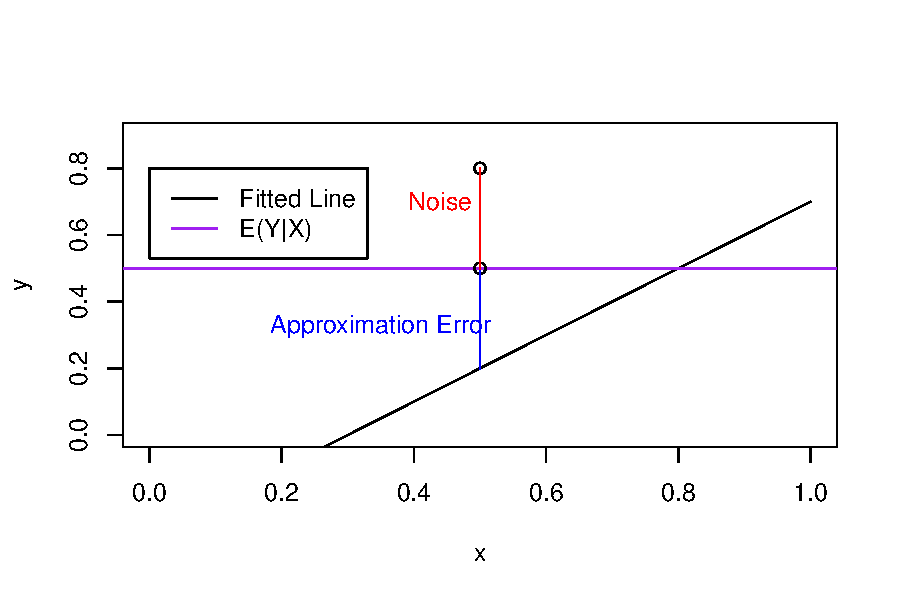
\includegraphics[width=\columnwidth]{decompLinear.pdf}}
\caption{Linear example of the modelling equation decomposition}
\label{decompLinear}
\end{center}
\end{figure}


\pagebreak

\begin{figure}[!h]
\begin{center}
\centerline{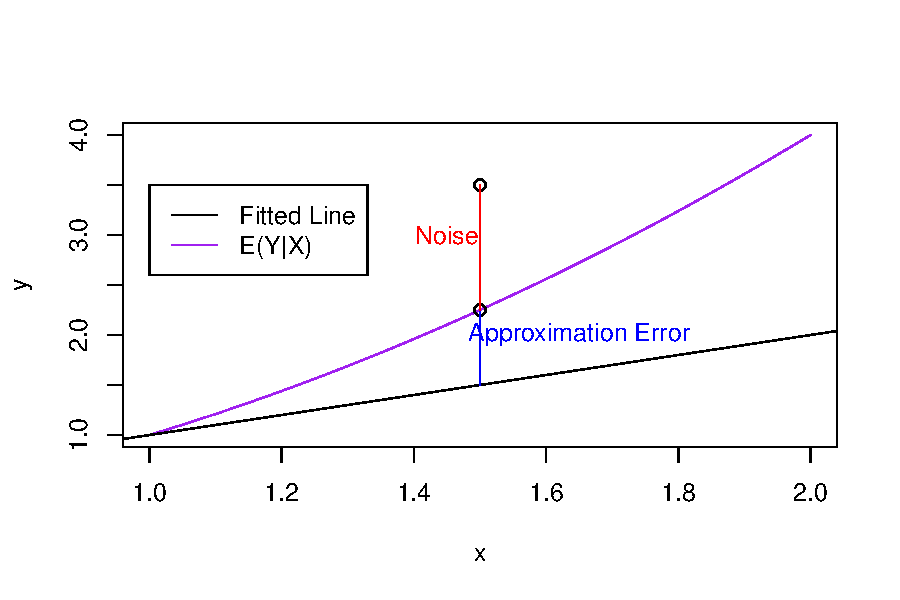
\includegraphics[width=\columnwidth]{decompNonLinear.pdf}}
\caption{Non-linear example of the modelling equation decomposition}
\label{decompNonLinear}
\end{center}
\end{figure}

The purpose of linear regression extends beyond modeling an assumed linear relationship between a response and predictor. In general, even in the presence of non-parametric components, linear regression can extract the parametric part of the surface of a response to derive inferences on parameters \cite{BBBGPTZZ2014}. 

The key difference between the cases illustrated in \cref{decompLinear} and \cref{decompNonLinear} is that when the linear assumption is violated, the approximation error also considers the deviation from linearity in the decomposition and can be considered the non-linearity term \cite{BBBGPTZZ2014}. 

Though not independent, the non-linearity term is uncorrelated with predictors since it is the population residual of the regression of $\mathbb{E}(Y|\textbf{x})$ \cite{BBBGPTZZ2014}.

\begin{lemma}
\label{lem:subgaussianNoise}
(Subgaussian Noise) $\exists \sigma < \infty$ where $\rho_{\lambda} \geq 1$ such that the following subgaussian noise bound occurs almost surely:
$$\mathbb{E}[exp\{(\eta) noise(\textbf{x})\} | \textbf{x}] \leq exp\{\eta^2\sigma^2/2 \}, \quad \forall \eta \in \mathbb{R}$$

This condition is satisfied in the case when the response noise is normally distributed, i.e., $\epsilon(\textbf{x}) \sim N(0, \sigma^2)$ \cite{HKZ2014}.
\end{lemma}

\begin{definition}
\label{def:ridgeEstReg}
The ridge estimator $\beta_{\lambda}$ is the minimizer of the regularized MSE, i.e.,
\begin{align*}
    \beta_{\lambda} &= \arg \min_w \mathbb{E}[(\langle w, \textbf{x} \rangle - y)^2] + \lambda||w||^2 \\
    &= (\Sigma + \lambda I)^{-1} \mathbb{E}[\textbf{x}y]
\end{align*}
\end{definition}

\begin{definition}
\label{def:approxErrorReg}
The approximation error of $\beta_{\lambda}$, from \cref{def:ridgeEstReg}, is 
\begin{align*}
    approx_{\lambda}(\textbf{x}) &= \mathbb{E}[y|\textbf{x}] - \langle \beta_{\lambda}, \textbf{x} \rangle\\
    &= \alpha_{\lambda}(\textbf{x})
\end{align*}
\end{definition}

\begin{lemma}
\label{lem:boundedApproxError}
(Bounded Approximation Error) $\exists b_{\lambda} < \infty$ where $b_{\lambda} \geq 1$ such that the following bounded approximation error occurs almost surely:
\begin{align*}
    \dfrac{||(\Sigma + \lambda I)^{-1/2}\textbf{x}\alpha_{\lambda}(\textbf{x})||^2}{\sqrt{\mathbb{E}[||(\Sigma + \lambda I)^{-1/2}\textbf{x}||^2]}} &\leq \dfrac{||(\Sigma + \lambda I)^{-1/2}\textbf{x}\alpha_{\lambda}(\textbf{x})||^2}{\sqrt{d_{1, \lambda}}} \\
    &\leq b_{\lambda}
\end{align*}
\cite{HKZ2014}.
\end{lemma}



\subsection{Dimensions of the Covariate}

The most effective dimensions of \textbf{x} depend on the eigenvalues of $\Sigma$, as defined in \cref{prop:eigval}, and the ridge regularization parameter $\lambda$, as chosen when solving \cref{def:ridgeEst}. 

\begin{definition}
\label{def:dimensions}
The effective dimensions of \textbf{x} are
$$d_{p, \lambda} = \sum_j \bigg( \dfrac{\lambda_j}{\lambda_j + \lambda} \bigg)^p, \qquad p \in \{1, 2\}$$
\end{definition}

\begin{remark}
$d_{2, \lambda} \leq d_{1, \lambda}$
\end{remark}

\begin{remark}
In the special case that $\lambda \longrightarrow \infty$, define the dimensions as $\Tilde{d}_{1, \lambda} = max\{d_{1, \lambda}, 1\}$
\end{remark}

\begin{definition}
\label{def:whitening}
The main condition requires that the squared length of $\textbf{x}$ is less
than or equal to a constant factor greater than its expectation. Define the expectation of the $\lambda$-whitening mapping when $\lambda > 0$ as 
\begin{align*}
    \mathbb{E}[||(\Sigma + \lambda I)^{-1/2}x||^2] &= tr[(\Sigma + \lambda I)^{-1/2} \Sigma (\Sigma + \lambda I)^{-1/2}] \\
    &= \sum_j \bigg( \dfrac{\lambda_j}{\lambda_j + \lambda} \bigg) \\
    &= d_{1, \lambda}
\end{align*}
\end{definition}

\begin{lemma}
\label{lem:boundedLeverage}
(Bounded Statistical Leverage) $\exists$ finite $\rho_{\lambda} \geq 1$ such that almost surely:
\begin{align*}
    \dfrac{||(\Sigma + \lambda I)^{-1/2}x||^2}{\sqrt{\mathbb{E}[||(\Sigma + \lambda I)^{-1/2}x||^2]}} &\leq \dfrac{||(\Sigma + \lambda I)^{-1/2}x||^2}{\sqrt{d_{1, \lambda}}}\\
        &\leq \rho_{\lambda}
\end{align*}

where the first inequality follows from \cref{def:whitening} \cite{HKZ2014}.
\end{lemma}



\pagebreak


\section{Random Design Setup for Ridge Regression}

Recall the two previously defined ridge estimators. 
\begin{itemize}
    \item $\hat{\beta}_{\lambda}$ as the estimator for the empirical MSE from \cref{def:ridgeEst}
    \item $\beta_{\lambda}$ as the estimator for the regularized MSE from \cref{def:ridgeEstReg}
\end{itemize}

\begin{remark}
It is important to note that in the case of a fixed design, $\hat{\beta}_{\lambda}$ is an unbiased estimator of $\beta_{\lambda}$, i.e.,
$$\mathbb{E}[\hat{\beta}_{\lambda}] = \beta_{\lambda}$$
This is not true in a random design setting, and using a biased estimator may lead to errors in the analysis. To prevent these errors, it is beneficial to use a different estimator. \cite{HKZ2011}
\end{remark}

\begin{definition}
\label{def:condExpBeta}
Another estimator can be defined as the conditional expectation of $\hat{\beta}_{\lambda}$ given $\textbf{x}_1, \textbf{x}_2...\textbf{x}_n$ is: 
\begin{align*}
    \Bar{\beta}_{\lambda} &= \mathbb{E}[\hat{\beta}_{\lambda} | \textbf{x}_1, \textbf{x}_2...\textbf{x}_n] \\
    &= (\hat{\Sigma} + \lambda I)^{-1}\hat{\mathbb{E}}[\textbf{x} \mathbb{E}[y|\textbf{x}]]
\end{align*}
\end{definition}

\begin{definition}
\label{def:biases}
Using \cref{def:excessMSE}, define the (1) regularization bias, (2) random design bias, and (3) variance as:
\begin{align}
    \epsilon_{rg} &= ||\beta_{\lambda} - \beta||^2_{\Sigma} \\
    \epsilon_{bs} &= ||\Bar{\beta}_{\lambda} - \beta_{\lambda}||^2_{\Sigma} \\
    \epsilon_{vs} &= ||\hat{\beta}_{\lambda} - \Bar{\beta}_{\lambda}||^2_{\Sigma}
\end{align}
\end{definition}

The main result provides strict upper bounds for the regularization bias, random design bias, and variance individually. These bounds can be used to create an upper bound for ridge regression in a random design setting. 

Finding this ridge bound will require a generic quantity that bounds the excess MSE of the empirical MSE estimator $\hat{\beta}_{\lambda}$ over the minimum estimator $\beta$. 

Using \cref{def:biases}, the following random design decomposition provides an upper bound on ridge regression in the randomized setting. 
\begin{proposition}
\label{prop:decomp}
\begin{align*}
    ||\hat{\beta}_{\lambda} - \beta||^2_{\Sigma} &\leq \epsilon_{rg} + \epsilon_{bs} + \epsilon_{vr} + 2(\sqrt{\epsilon_{rg}\epsilon_{bs}} + \sqrt{\epsilon_{rg}\epsilon_{vr}} \\
    &\qquad + \sqrt{\epsilon_{bs}\epsilon_{vr}})\quad,\\
    &\leq 3(\epsilon_{rg} + \epsilon_{bs} + \epsilon_{vr})
\end{align*}
\end{proposition}


\pagebreak



\section{Main Result}
The main result of the original paper concerns itself with the effect of errors on the covariance structure. 

This result depends on the following assumptions:

\begin{itemize}
    \item Assume \cref{lem:subgaussianNoise}, \cref{lem:boundedApproxError}, \cref{lem:boundedLeverage} are true
    \item Assume that the sample size n has a lower bound of $n \geq 6 \rho^2_{\lambda} d_{1, \lambda} (log(\Tilde{d}_{1,\lambda}) + t)$.
\end{itemize}

\begin{theorem}
\label{thm:ridge}
Choose a constant ridge parameter $\lambda \geq 0$. Choose $t > max\{0, 2.6 - log(\Tilde{d}_{1,\lambda})\}$.

Given these assumptions, the equations and inequalities below hold true with a probability of at least $1 - 4e^{-t}$:
\begin{enumerate}
    \item \textbf{Spectral norm error of $\hat{\Sigma} + \lambda I$}
    \begin{align*}
        ||(\Sigma + \lambda I)^{1/2}(\hat{\Sigma} + \lambda I)^{-1}(\Sigma + \lambda I)^{1/2}|| \leq (1 - \delta_s)^{-1}
    \end{align*}
    where:
    \begin{align*}
        \delta_s &= \sqrt{\dfrac{4 \rho^2_{\lambda} d_{1, \lambda} (log(\Tilde{d}_{1, \lambda}) + t)}{n}} \\
        &\qquad + \dfrac{2 \rho^2_{\lambda} d_{1, \lambda} (log(\Tilde{d}_{1, \lambda}) + t)}{3n}
    \end{align*}
    and $\delta_s \leq 0.93 < 1$
    \item \textbf{Frobenius norm error of $\hat{\Sigma}$}
    \begin{align*}
        ||(\Sigma + \lambda I)^{1/2}(\hat{\Sigma} + \Sigma)^{-1}(\Sigma + \lambda I)^{1/2}||_F \leq \delta_f \sqrt{d_{1, \lambda}} 
    \end{align*}
    where:
    \begin{align*}
        \delta_f &= \sqrt{\dfrac{\rho^2_{\lambda} d_{1, \lambda} - d_{1, \lambda}/d_{1, \lambda}}{n}}(1 + \sqrt{8t}) \\
        &\qquad + \dfrac{4 \sqrt{\rho^2_{\lambda} d_{1, \lambda} - d_{1, \lambda}/d_{1, \lambda} t}}{3n}
    \end{align*}
    \item \textbf{Regularization effect}
    \begin{align*}
        \epsilon_{rg} \leq \sum_j \dfrac{\lambda_j}{(\frac{\lambda_j}{\lambda} + 1)^2}\beta_j^2
    \end{align*}
    In the special OLS case when $\lambda = 0$, we have $\epsilon_{rg} = 0$
    \item \textbf{The Effect of Bias due to Random Design}
    \begin{align*}
        \epsilon_{bs} &\leq \dfrac{2}{(1 - \delta_s)^2} \bigg(\dfrac{\mathbb{E}[||(\Sigma+\lambda I)^{-1/2} (x \alpha_{\lambda}(x) - \lambda \beta_{\lambda})||^2]}{n} \\
        &\qquad (1 + \sqrt{8t})^2 + \dfrac{16(b_{\lambda}\sqrt{d_{1, \lambda}} + \sqrt{\epsilon_{rg}})^2 t^2}{9n^2} \bigg) \\
        &\leq \dfrac{4}{(1 - \delta_s)^2} \bigg( \dfrac{\rho^2_{\lambda} d_{1, \lambda} \mathbb{E}[\alpha_{\lambda}(x)^2] + \epsilon_{rg}}{n} (1 + \sqrt{8t})^2 \\
        &\qquad + \dfrac{(b_{\lambda}\sqrt{d_{1, \lambda}} + \sqrt{\epsilon_{rg}})^2t^2}{} \bigg)
    \end{align*}
    \item \textbf{The Effect of Noise}
    \begin{align*}
        \epsilon_{vr} &\leq \dfrac{\sigma^2 (d_{2, \lambda} + \sqrt{d_{1, \lambda}d_{2, \lambda}} \delta_f)}{n (1 - \delta_s)^2} + \dfrac{2 \sigma^2 t}{n (1 - \delta_s)}\\
        &\qquad  + \dfrac{2\sigma^2 \sqrt{(d_{2, \lambda} + \sqrt{d_{1, \lambda}d_{2, \lambda}} \delta_f) t}}{n (1 - \delta_s)^{3/2}}
    \end{align*}
\end{enumerate}
\cite{HKZ2014}
\end{theorem}

Note that for this theorem, the bound on n implies that n should be sufficiently large compared to some constant factor of the dimensions of the covariate x. 

As previously stated, this result is used to provide upper bounds on $\epsilon_{vr}, \epsilon_{rg}, \epsilon_{bs}$, which will imply an upper bound on $||\hat{\beta}_{\lambda} - \beta||^2_{\Sigma}$.

\begin{proposition}
\label{prop:ridgeBound}
The bound on $||\hat{\beta}_{\lambda} - \beta||^2_{\Sigma}$ using results 3, 4, and 5 from \cref{thm:ridge} is given by the following:
\begin{align*}
    ||\hat{\beta}_{\lambda} - \beta||^2_{\Sigma} &\leq ||\beta_{\lambda} - \beta||^2_{\Sigma} \\
    &\qquad + \mathcal{O}\bigg(\dfrac{\rho^2_{\lambda} d_{1, \lambda} \mathbb{E}[\alpha(x)^2]}{n} \\
    &\qquad + \dfrac{ (\rho^2_{\lambda} d_{1, \lambda} +1 )||\beta_{\lambda} - \beta||^2_{\Sigma} + \sigma^2 d_{2, \lambda} }{n} \bigg)
\end{align*}
\cite{HKZ2014}
\end{proposition}

\subsection{Significance of Results}

\textbf{The Effects of Errors}: Though these results appear rather complex, the simple implication is that the accuracy of $\hat{\Sigma}$ has a fairly mild effect on the bound. 

Specifically, it appears through constant factors of the spectral and Frobenius norm errors from \cref{thm:ridge}, where the terms are decreasing as sample size increases, therefore contributing to lower-order terms overall.

\textbf{The Effect of Approximation Errors:} The effect of approximation error $\epsilon_{bs}$ is an isolated term in \cref{prop:decomp}. Its upper bound is the addition of the scaling of approximation errors depending on $\rho_\lambda d_{1,\lamda}$ with some stochastic noise. This scaling term also contributes to lower-order terms overall and approaches 1 as $n \rightarrow \infty$ 

\textbf{Significance:} Based on the above remarks, the conclusion is that the ridge estimators behave similarly under fixed and random design settings, even though there is an influence of approximation error under random design. 

This is because of the upper bound which tells us that the effect is second order and converges to a constant given sufficiently large sample sizes. This phenomenon will be explored in the proceeding section through a simple linear regression example.






\section{Numerical Studies}
The fixed design setting is restricted to observations made for controlled values of $X$, so there is no statistical validity to out-of-sample predictions. For experimenters, it may not always be feasible to control the predictors. In an observational study, certain groups may be more frequently observed than others, since the covariates follow their own natural distribution. 

This introduces a bias or approximation error on top of random noise when attempting to model the relationship between predictors and responses. To further understand the effects of errors in a random design setting, where covariance structures are completely unknown, it is necessary to highlight its differences with a fixed design setting.


\subsection{Simple Linear Regression in a Fixed vs Random Design Setting}
For simplicity in the following example, consider a single explanatory variable for an ordinary least squares regression model, which is a special case of ridge regression where the regularization parameter $\lambda=0$.

A population with predictors $X$ and responses $Y$ has the linear relationship $Y=\beta X+\epsilon$, where $\epsilon \sim \mathcal{N}(0,\sigma^2)$.

\textbf{Assumptions:} 
\begin{itemize}
    \item Assume in both cases that the noise term $\epsilon$ is normally distributed
    \item For fixed values of $X$:  $\mathbb{E}(\epsilon)=0$, $\text{var}(\epsilon)=\sigma^2$ and $\text{cov}(\epsilon_i,\epsilon_j)=0$
    \item When the predictor is random, it can only be assumed conditionally that $\mathbb{E}(\epsilon|x)=0$ and $\text{var}(\epsilon|x)=\sigma^2$ for particular outcomes of $X$
    \begin{itemize}
        \item This is a key assumption in random design analysis because it ensures similar properties to a fixed design setting that would allow the covariates to be treated as if they were deterministic
    \end{itemize}
\end{itemize}

\cite{HGL2011}

\textbf{The Fixed Design Setting:} Treat $X$ as deterministic, meaning values of $X$ are controlled for in this particular experiment. 


To simulate a fixed design setting, let the true value of the coefficient $\beta$ be 1, and suppose a sequence of 100 numbers between -2 and 2 is fit to the response variable with added noise from the standard normal distribution. 


The code for this section is found in \cref{code:fixed}. \cref{table:linRegFixedTable}, \cref{linRegFixed}, and \cref{linRegFixedQQ} summarize an instance of this linear regression model in a fixed design setting.


\begin{table}[!h]
\vskip 0.15in
\begin{center}
\begin{small}
\begin{sc}
\begin{tabular}{lccc}
\toprule
Term & Estimate & Std. Error & p. Value \\
\midrule
(Intercept) & 0.1088874 & 0.0902675 & 0.2306156 \\
Explanatory & 0.9888363 & 0.0773960 & 0.0000000\\
\bottomrule
\end{tabular}
\end{sc}
\end{small}
\end{center}
\caption{Linear regression model in a fixed design setting}
\label{table:linRegFixedTable}
\vskip -0.1in
\end{table}

\begin{figure}[!h]
\vskip 0.2in
\begin{center}
\centerline{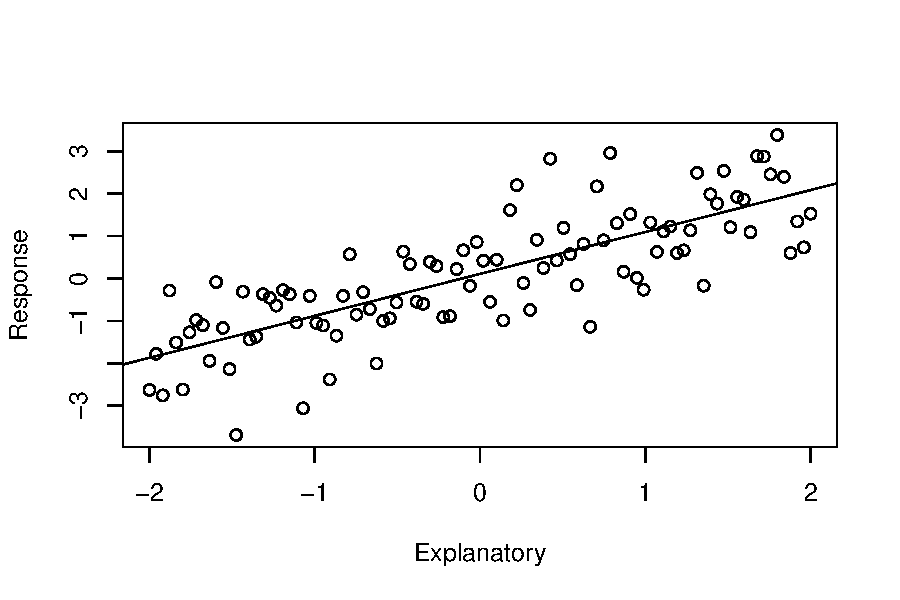
\includegraphics[width=\columnwidth]{fixedReg.pdf}}
\caption{Linear regression model in a fixed design setting}
\label{linRegFixed}
\end{center}
\vskip -0.2in
\end{figure}

\begin{figure}[!h]
\vskip 0.2in
\begin{center}
\centerline{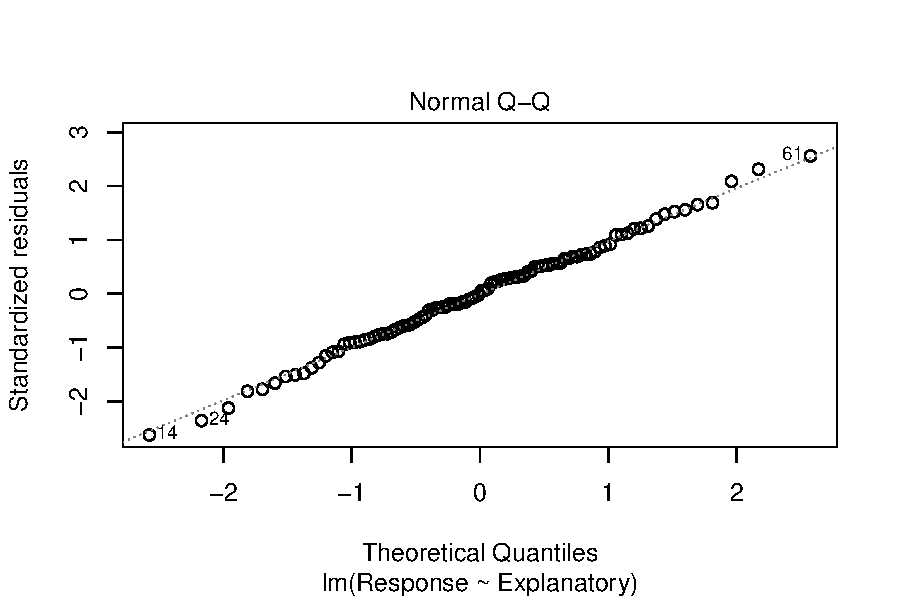
\includegraphics[width=\columnwidth]{fixedQQ.pdf}}
\caption{Linear regression model normal quantile plot in a fixed design setting}
\label{linRegFixedQQ}
\end{center}
\vskip -0.2in
\end{figure}


\textbf{The Random Design Setting:} Treat $X$ as random, meaning values of $X$ are not controlled for and are determined jointly with $Y$ and $\epsilon$ for each sample in the experiment. 

To simulate a random design setting, suppose values of $X$ are drawn from a standard normal distribution. Let the true value of the coefficient $\beta$ also be 1, and fit the model with added noise from the standard normal distribution.

The code for this section is found in \cref{code:random}. \cref{table:linRegRandomTable}, \cref{linRegRandom}, and \cref{linRegRandomQQ} summarize an instance of this linear regression model in a random design setting.

\begin{table}[!h]
\vskip 0.15in
\begin{center}
\begin{small}
\begin{sc}
\begin{tabular}{lccc}
\toprule
Term & Estimate & Std. Error & p. Value \\
\midrule
(Intercept) & -0.0376926 & 0.0969873 & 0.6983896 \\
Explanatory & 0.9989396 & 0.1077270 & 0.0000000 \\
\bottomrule
\end{tabular}
\end{sc}
\end{small}
\end{center}
\caption{Linear regression model in a random design setting}
\label{table:linRegRandomTable}
\vskip -0.1in
\end{table}


\begin{figure}[!h]
\vskip 0.2in
\begin{center}
\centerline{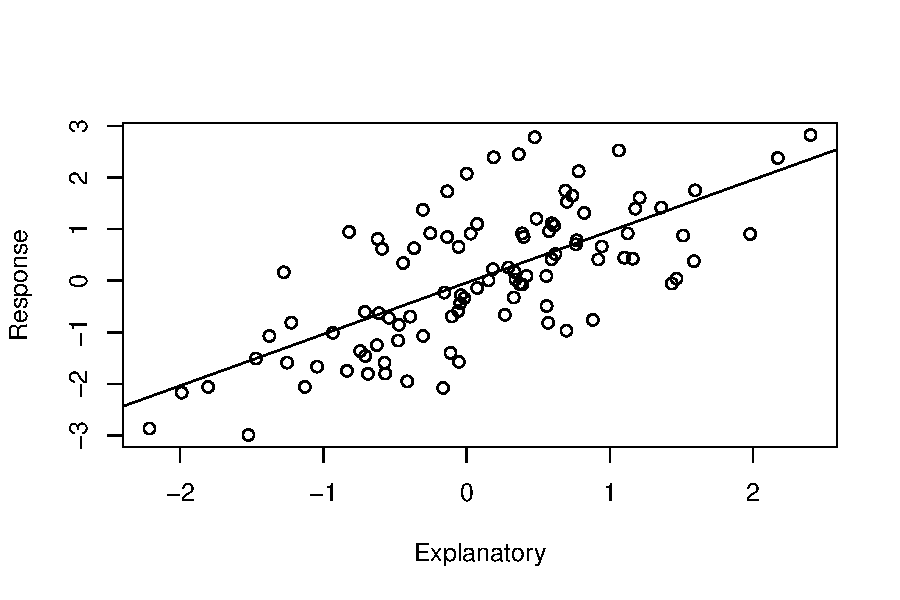
\includegraphics[width=\columnwidth]{randomReg.pdf}}
\caption{Linear regression model in a random design setting}
\label{linRegRandom}
\end{center}
\vskip -0.2in
\end{figure}

\begin{figure}[!h]
\vskip 0.2in
\begin{center}
\centerline{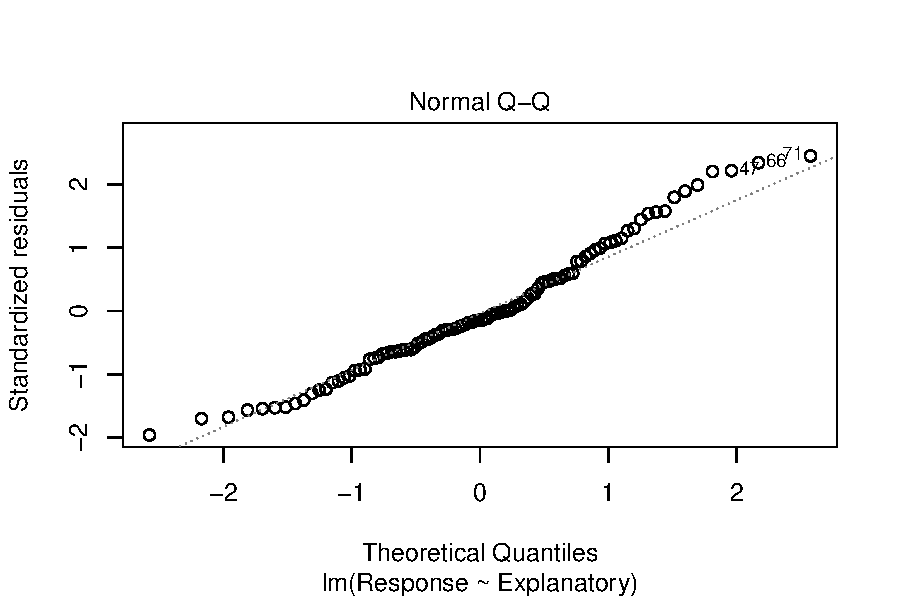
\includegraphics[width=\columnwidth]{randomQQ.pdf}}
\caption{Linear regression model normal quantile plot in a random design setting}
\label{linRegRandomQQ}
\end{center}
\vskip -0.2in
\end{figure}


With a sample size of 100, the estimated coefficient in both instances is statistically significant and very close to the true value 1 (from the tables, note that the p-value $<$ 2e-16). 

The plots vary slightly since $X$ in the random design setting follows a normal distribution and is not fixed. This leads to more observations being made towards the center; however, the model was still able to accurately fit the relationship between the response and explanatory variables. 

The normal quantile plots of the residuals indicate that the distribution of errors in both instances is relatively normal. This is all evidence to suggest that the error effect is indeed second order for sufficiently large sample sizes. To further demonstrate this conclusion, Monte Carlo simulations can help explain the impact of the uncertainty between different samples.


\subsection{Monte Carlo Simulations}
The simulations explained above were repeated to obtain estimated values of $\beta$. The distribution of these estimates are shown below for the random design setting with increasing numbers of repeated sampling (N). The code for these simulations can be found in \cref{code:montecarlo}.

\begin{figure}[!h]
\begin{center}
\centerline{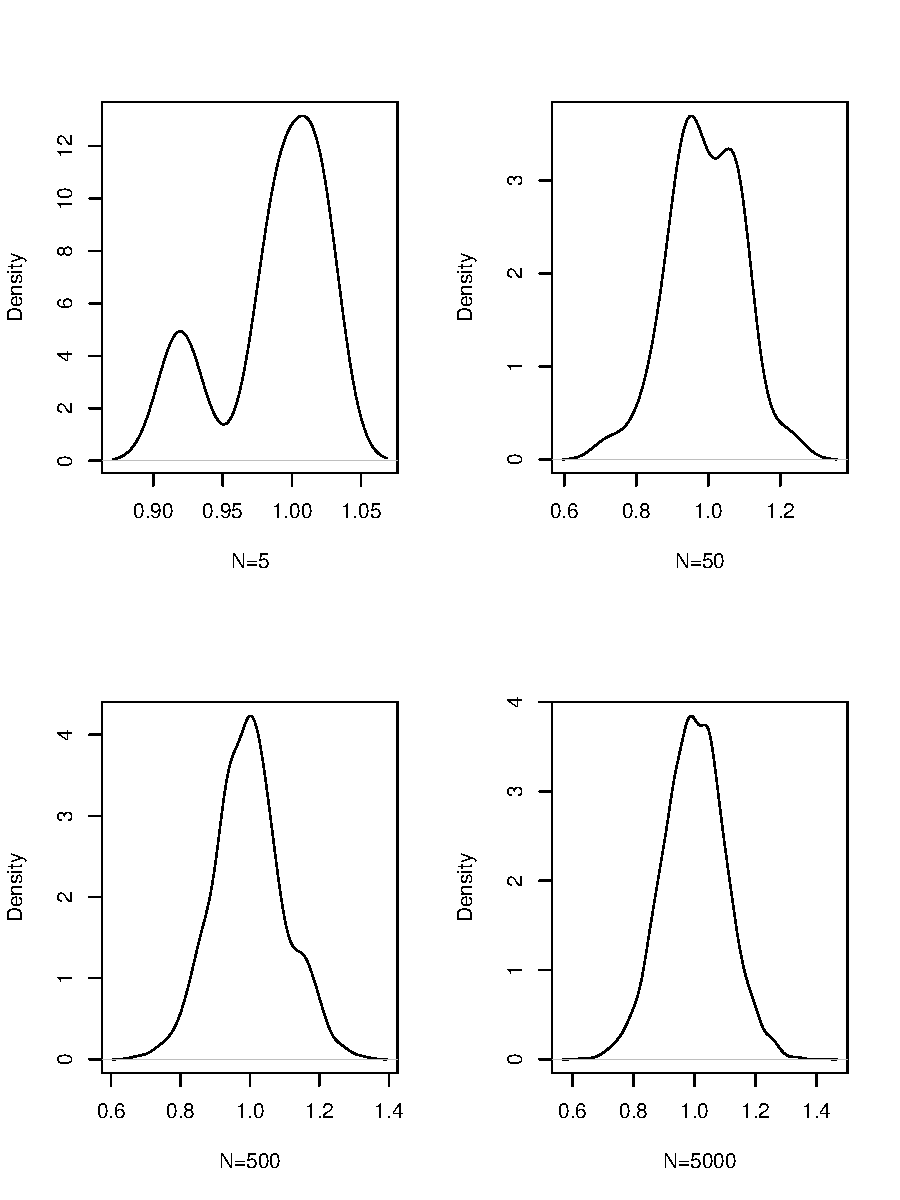
\includegraphics[width=\columnwidth]{montecarloRandom.pdf}}
\caption{Distribution of Monte Carlo simulation estimations}
\label{montecarloRandom}
\end{center}
\vskip -0.2in
\end{figure}

\cref{montecarloRandom} illustrates how the distribution of sample estimates of $\beta$ converges to a normal distribution centered at the true value which is 1. 

For further insight, the same simulation for both the fixed and random design setting was repeated 10 000 times to compare the distribution of the estimated regression coefficient.

\pagebreak

\begin{figure}[!h]
\begin{center}
\centerline{\includegraphics[width=\columnwidth]{montecarlo10000.pdf}}
\caption{Distribution of Monte Carlo simulation estimations}
\label{montecarlo10000}
\end{center}
\vskip -0.2in
\end{figure}

Based on the Monte Carlo simulations in \cref{montecarlo10000}, the distributions of estimated values in both the fixed and random setting appear to follow a normal curve centered at the true value of $\beta$, which is 1. 

This is evidence supporting the claim that the estimator behaves similarly under fixed and random designs, with the main difference being the lack of error in $\hat{\Sigma}$ under a fixed setting and the influence of bias and approximation error under random design. 

This difference is highlighted by the variation seen in the distribution of $\hat{\beta}$, with there being a slightly larger spread of estimated values in the random setting. This illustrates how the scaling of the bounded statistical leverage $\rho_\lambda^2d_{1,\lambda}$ with $\lambda$ is crucial in controlling the effect of errors in random design settings when compared to fixed.
\cite{HKZ2014}


\section{Limitations}
One of the biggest limitations of \cref{thm:ridge} is the restriction on sample size because it will only hold if the sample size is sufficiently large, and will fail otherwise. The rest of the assumptions are not overly restrictive, as the numerical study has shown that scaling the bounded statistical leverage is necessary in order for the results to hold. 

This paper analyzes a fixed effect model where the regression coefficients are assumed to be deterministic. In the case where effects may be random, however, the impact of errors may be more substantial so the results of the original work may not hold under these conditions.

\section{Future Directions}
A future research direction could be to perform similar analyses for Lasso regression, or ElasticNet regression. The original paper concludes that the effect of ridge regression errors are similar in random design vs fixed design settings, but it may be beneficial to also understand the impact of different regularization terms on the regression function. 

Another future research direction for this paper might interest itself in determining whether or not a random design setting behaves similar to a fixed design setting when both the predictors and regression slopes are random. 





%%%%%%%%%%%%%%%%%%%%%%%%%%%%%%%%%%%%%%%%%%%%%%%%%%%%%%%%%%%%%%%%%%%%%%%%%%%%%%%
%%%%%%%%%%%%%%%%%%%%%%%%%%%%%%%%%%%%%%%%%%%%%%%%%%%%%%%%%%%%%%%%%%%%%%%%%%%%%%%
% References
%%%%%%%%%%%%%%%%%%%%%%%%%%%%%%%%%%%%%%%%%%%%%%%%%%%%%%%%%%%%%%%%%%%%%%%%%%%%%%%
%%%%%%%%%%%%%%%%%%%%%%%%%%%%%%%%%%%%%%%%%%%%%%%%%%%%%%%%%%%%%%%%%%%%%%%%%%%%%%%
\newpage
\onecolumn
% In the unusual situation where you want a paper to appear in the
% references without citing it in the main text, use \nocite
\nocite{RT2017}
\bibliography{stad80_final_project}
\bibliographystyle{icml2022}






%%%%%%%%%%%%%%%%%%%%%%%%%%%%%%%%%%%%%%%%%%%%%%%%%%%%%%%%%%%%%%%%%%%%%%%%%%%%%%%
%%%%%%%%%%%%%%%%%%%%%%%%%%%%%%%%%%%%%%%%%%%%%%%%%%%%%%%%%%%%%%%%%%%%%%%%%%%%%%%
% APPENDIX
%%%%%%%%%%%%%%%%%%%%%%%%%%%%%%%%%%%%%%%%%%%%%%%%%%%%%%%%%%%%%%%%%%%%%%%%%%%%%%%
%%%%%%%%%%%%%%%%%%%%%%%%%%%%%%%%%%%%%%%%%%%%%%%%%%%%%%%%%%%%%%%%%%%%%%%%%%%%%%%
\appendix
\onecolumn
\section{Appendix}

\subsection{The Fixed Design Setting Code}
\label{code:fixed}
\begin{lstlisting}[language=R]
    library(tidyverse)
    set.seed(1)
    Explanatory <- seq(-2,2,length.out=100)
    Response <- Explanatory + rnorm(length(Explanatory))
    model <- lm(Response~Explanatory)
    model_summary <- model %>% broom::tidy() %>% kable()
    
    # PLOT 
    par(mfrow=c(1,2))
    plot(Response~Explanatory)
    abline(model)
    plot(model,which = 2)
\end{lstlisting}


\subsection{The Random Design Setting Code}
\label{code:random}
\begin{lstlisting}[language=R]
    set.seed(1)
    Explanatory <- rnorm(100)
    Response <- Explanatory + rnorm(length(Explanatory))
    model <- lm(Response~Explanatory)
    model_summary <- model %>% broom::tidy() %>% kable()
    
    # PLOT
    par(mfrow=c(1,2))
    plot(Response~Explanatory)
    abline(model)
    plot(model, which=2)
\end{lstlisting}


\subsection{Decomposition Plot Code}
\label{code:decomp}
\begin{lstlisting}[language=R]
    ## Non Linear data
    set.seed(1)
    curve(x^2,from=1,to=2, xlab="x",ylab="y", col="purple")
    abline(0,1)
    points(c(1.5,1.5),c(3.5,1.5^2))
    legend(1,3.5, legend=c("Fitted Line", "E(Y|X)"),
           col=c("black", "purple"), lty=1)
    lines(c(1.5,1.5),c(1.5,1.5^2), col="blue")
    lines(c(1.5,1.5),c(1.5^2,3.5), col="red")
    text(1.65,2,label = "Approximation Error", col="blue")
    text(1.45,3,label = "Noise",col="red")
    
    ## Linear data
    curve(1*x,from=0,to=1, col="purple",ylab="y")
    abline(h=0.2)
    points(c(.5,.5),c(.5,0.8))
    legend(0,0.8, legend=c("Fitted Line", "E(Y|X)"),
           col=c("black", "purple"), lty=1)
    lines(c(.5,.5),c(0.2,0.5), col="blue")
    lines(c(.5,.5),c(0.5,0.8), col="red")
    text(.645,.3,label = "Approximation Error", col="blue")
    text(.45,.7,label = "Noise",col="red")
\end{lstlisting}



\subsection{Monte Carlo Simulations Code}
\label{code:montecarlo}
\begin{lstlisting}[language=R, breaklines=true]
    set.seed(1)
    N <- 10000
    X <- seq(-3,3,length.out=100)
    beta_fixed <- vector()
    for (i in 1:N){
      y <- X +rnorm(100)
      model <- lm(y~X)
      beta_fixed[i] <- model$coefficients[2]
    }
    beta_random <- vector()
    for (i in 1:N){
      X <- rnorm(100)
      y <- X+rnorm(100)
      model <- lm(y~X)
      beta_random[i] <- model$coefficients[2]
    }
    
    par(mfrow=c(1,2))
    plot(density(beta_fixed),cex.main=1, main="Distribution of Estimated Coefficients - Fixed X", xlab = "N=10000")
    plot(density(beta_random),cex.main=1, main="Distribution of Estimated Coefficients - Random X", xlab = "N=10000")
\end{lstlisting}

\end{document}


% This document was modified from the file originally made available by
% Pat Langley and Andrea Danyluk for ICML-2K. This version was created
% by Iain Murray in 2018, and modified by Alexandre Bouchard in
% 2019 and 2021 and by Csaba Szepesvari, Gang Niu and Sivan Sabato in 2022. 
% Previous contributors include Dan Roy, Lise Getoor and Tobias
% Scheffer, which was slightly modified from the 2010 version by
% Thorsten Joachims & Johannes Fuernkranz, slightly modified from the
% 2009 version by Kiri Wagstaff and Sam Roweis's 2008 version, which is
% slightly modified from Prasad Tadepalli's 2007 version which is a
% lightly changed version of the previous year's version by Andrew
% Moore, which was in turn edited from those of Kristian Kersting and
% Codrina Lauth. Alex Smola contributed to the algorithmic style files.
